\documentclass[a4paper,10pt]{article}

\usepackage[brazil]{babel}
\usepackage[utf8]{inputenc}
\usepackage[T1]{fontenc}

\usepackage{geometry}
 \geometry{
 a4paper,
 total={170mm,257mm},
 left=20mm,
 top=20mm,
 right=20mm,
 }

%\usepackage[bottom=2cm,top=2cm,left=1.5cm,right=2cm]{geometry}	
\usepackage[hidelinks]{hyperref}
\usepackage{graphicx}
\usepackage{tikz}
\usepackage{amssymb}
\usepackage{indentfirst}
\usepackage{multirow}
\usepackage{rotating}
\usepackage{tabularx}
\usepackage{ragged2e}
\usepackage{longtable}
\usepackage{lscape}
\pagestyle{headings}
\newcommand{\SPNC}{$\mathcal{SPN}^{\mathcal{C}}$}
\newcommand{\place}{\textit{place}}

\renewcommand{\baselinestretch}{1.5} 

% {\setstretch{1.0}\color{blue}
% \lipsum[2]
% }

\title{Sistema Imune Inato - Uma Abordagem com Redes de Petri}

%\author{Elvis Hernandes Ribeiro}
\author{Elvis Hernandes Ribeiro\thanks{Financiado por uma bolsa da Fapemig}}


\begin{document}

    \maketitle

    % 		Muitos fatores contribuem para a capacidade dos patógenos em estabelecer infecções persistentes, incluindo tanto 
% 		fatores hospedeiros quanto bacterianos. Uma infecção crônica pode ser consequência de um sistema imunológico debilitado, onde uma ou mais 
% 		células do sistema imune não estão realizando suas funções normalmente e certos agentes patogênicos parecem adaptados a explorar 
% 		as vulnerabilidades existentes. 
    \begin{abstract}				
		O entendimento de fenômenos complexos na Imunologia é um grande desafio para cientistas em vários campos da ci\^encia. 
		Nos últimos anos, Redes de Petri estão sendo usadas para modelagem de sistemas biológicos. Exemplos disso incluem 
		a modelagem de reações bioquímicas, de redes de interação proteica, de redes de regulação gênica, 
		modelagem do sistema imunológico, entre outros. 
		Neste trabalho, redes de Petri são utilizadas para modelar o papel de neutrófilos e macrófagos durante a resposta imune inata a uma infecção bacteriana. 
		Vários processos presentes nas respostas imunes são considerados e esses processos são modelados com transições estocásticas na rede de Petri. 
		Objetiva-se estudar, com as redes de Petri construídas, a importância do papel regulador do macrófago na resolução da resposta imune e os efeitos 
		de considerar a influência do dano tecidual na resposta imune. 
    \end{abstract}

    \newpage 
		\tableofcontents
    \newpage

    \section{Introdução}
    
		%Falar sobre infecções agudas e crônicas com a bactéria \textit{Staphylococcus aureus}.
		
		%Consultar Livro Imunobiologia de Janeway 
		
		O entendimento de fenômenos complexos na Imunologia é um grande desafio para cientistas em vários campos 
		da biologia, medicina e farmacologia \cite{Carvalho2015}. Os fenômenos biológicos relacionados às infecções e ao sistema imune 
		podem ser descritos por diversos tipos de modelos dentre os quais destaca-se: equações diferenciais ordinárias, 
		equações diferenciais parciais, modelos baseados em agentes, autômatos celulares, dinâmica de sistemas, 
		redes de Petri, entre outros. Todos esses modelos podem contribuir com o entendimento de mecanismos presentes 
		na interação entre o patógeno e o hospedeiro através da modelagem e simulação de diversos aspectos das 
		respostas imunes \cite{Carvalho2015}.  
		
		Para muitos patógenos bacterianos, o sistema imunológico do hospedeiro elimina completamente as bactérias invasoras 
		e a infecção é resolvida, ou seja, a inflamação e os danos teciduais cessam. No entanto, em alguns casos, devido 
		a vários fatores como doenças pré-existentes, imunidade baixa, entre outros, as bactérias evadem o sistema imune 
		e estabelecem um ambiente favorável para a persistência (cenário esse que caracteriza uma infecção crônica) \cite{Grant2013}. 
		Em certos casos, essas infecções persistentes são assintomáticas 
		por longos períodos de tempo, mas podem sofrer reativação futura em doença clinicamente significativa, ou podem estar 
		associadas a malignidade ou disseminação subsequente da doença \cite{Grant2013}. Alternativamente, algumas infecções persistentes 
		resultam em sintomas crônicos clinicamente aparentes. Nesses casos, mesmo o tratamento padrão com antibióticos muitas 
		vezes não consegue esterilizar eficazmente essas infecções, e cursos prolongados ou repetidos de antibióticos 
		são necessários para a erradicação bem sucedida. Ao extremo, a supressão crônica ao longo da vida com antibióticos 
		pode ser necessária na ausência de erradicação \cite{Grant2013}.		
		
		Muitos fatores contribuem para a capacidade dos patógenos em estabelecer infecções persistentes, incluindo tanto 
		fatores hospedeiros quanto bacterianos. Certos agentes patogênicos parecem unicamente adaptados para escapar do 
		sistema imune do hospedeiro e persistir em indivíduos infectados por décadas na ausência de sintomas como, por exemplo, 
		\textit{Mycobacterium tuberculosis} ou \textit{Salmonella Typhi}. Outros patógenos como \textit{Pseudomonas aeruginosa} 
		ou \textit{Escherichia coli} podem causar tanto sintomas agudos como crônicos, com alterações específicas no hospedeiro, 
		facilitando o estabelecimento de uma infecção persistente \cite{Grant2013}.
		%Bacteria adapt to environmental stresses imposed by the host by entering a different physiologic state. 
		%A key element of this different physiologic state is a non-replicating or slowly replicating growth rate, 
		%which may have the additional benefit of contributing to a pathogen’s defense against antibiotic exposure. 
		
		%Chronic conditions exhibit many of the same immune signatures of acute infection, including loss of barrier function, tissue destruction, and functional impairment, and are becoming increasingly prevalent worldwide (Karin et al., 2006)
		Uma condição crônica pode ser causada por uma infecção aguda como mostra o trabalho de Moraes \textit{et al} \cite{Fonseca2015} que ao estudar infecções 
		com \textit{Yesrsinia pseudotuberculosis} observaram que a infecção aguda teve um impacto de longa duração na estrutura e função do sistema imune do intestino \cite{Fonseca2015}. 
		
		Em muitos casos, infecções crônicas estão associadas com uma inflamação crônica. A inflamação crônica é caracterizada por repetidos ciclos de migração 
		de células do sistema imune, produção de substâncias pró-inflamatórias e dano tecidual que se não forem contidos pelo próprio sistema imune podem levar a 
		consequências graves para o paciente. Os macrófagos são uma das principais células responsáveis pela regulação dessa resposta pró-inflamatória através, 
		por exemplo, da produção de citocinas anti-inflamatórias, da fagocitose de células apoptóticas e da fagocitose de células de tecido mortas, entre outras ações. 
		Portanto, caso o papel regulador dos macrófagos esteja prejudicado por algum motivo, o resultado pode ser fatal. 
		Nesse caso, os macrófagos poderiam contribuir para a continuação da inflamação e do dano tecidual. 

		%Objetivo	
		Nos últimos anos, Redes de Petri estão sendo usadas para modelagem de sistemas biológicos. Exemplos disso incluem 
		a modelagem de reações bioquímicas, de redes de interação proteica, de redes de regulação gênica, 
		modelagem do sistema imunológico, entre outros. 
				
		Neste trabalho, redes de Petri são utilizadas para estudar comportamentos observados em infecções bacterianas que podem ser agudas ou crônicas.  
		O objetivo deste trabalho é estudar a importância do papel regulador do macrófago na resolução da resposta imune e os efeitos da influência do dano 
		tecidual na resposta imune. 		
				
		%No contexto da modelagem do sistema imunológico, destaca-se o trabalho de Rafael \textit{et al.} ...
		
% 		Outro trabalho relacionado é o trabalho de Jarrett \textit{et al.} \cite{Jarrett2015} que estuda a interação entre o 
% 		sistema imune, bactéria e inflamação através de equações diferenciais ordinárias. 
% 		O modelo é validado com experimentos de vacinação e imunomodulação. 
% 		Jarrett \textit{et al.} \cite{Jarrett2015} desenvolveram um modelo com os seguintes componentes: bactérias, a resposta pró-inflamatória 
% 		representando as citocinas pró-inflamatórias e células do sistema imune envolvidas nas respostas 
% 		Th1 e Th17 (IL-2, IL-12p70, IL-6, IL-17, TNF-$\alpha$, IL-1$\beta$, neutrophils), a resposta 
% 		anti-inflamatória de Th2 e Treg (IL-4 e IL-10) e a inflamação que é usada para representar 
% 		vários processos como um grande fluxo sanguíneo, danos celulares e uma sinalização pró-inflamatória. 
% 				 
% 		Jarrett \textit{et al.} \cite{Jarrett2015} obtiveram o resultado de inflamação crônica (quando a inflamação persiste em um nível elevado) 
% 		quando as seguintes mudanças de parâmetros foram efetuadas: 
% 		\begin{itemize}
% 		 \item 
% 		\end{itemize}
% %     decreasing the anti-inflammatory response rate, α2, representing a deficiency in the anti-inflammatory response;
% %     increasing the production of inflammation/damage due to the pro-inflammatory response, α3, representing an immune response more sensitive to its own cells;
% %     increasing the rate at which inflammation hinders the anti-inflammatory response, β2, representing blockage to anti-inflammatory cells and cytokines/chemokines;
% %     and decreasing the rate at which the anti-inflammatory response reduces inflammation, β3, representing an ineffectiveness of the anti-inflammatory cells (Fig. 2).
% %     
% 		Jarrett \textit{et al.} verificaram que 
				
		% Before a challenge, the immune system is maintained at a low level of activation with no active response and low levels of passive/innate response components (Delves & Roitt, 2000b). Under ideal circumstances, the interplay between the pro-inflammatory, anti-inflammatory and ‘inflammation’ components will bring the body back to a basal or healthy level.		
	
					
		%O problema com a inflamação não é com que frequência ela começa, mas com que frequência ela não diminui. Talvez nenhum fenômeno isolado contribua mais para a carga 
		% médica nas sociedades industrializadas do que a inflamação não resolvida. A inflamação não-resolvida não é uma causa primária de aterosclerose, obesidade, câncer, doença pulmonar obstrutiva crônica, asma, doença inflamatória intestinal, doença neurodegenerativa, esclerose múltipla ou artrite reumatóide, mas contribui significativamente para sua patogênese.

		%Esta revisão ilustrativa, mas não abrangente, começa descrevendo diferentes formas de inflamação não-resolvida. Discutimos então o dano dos tecidos não infectados como propagador da inflamação. Esta é uma questão conceitual crítica, porque os estímulos microbianos não estão implicados em muitas formas de inflamação crônica, e é instrutivo avaliar o valor adaptativo de nossa capacidade de lançar um processo de dano tecidual desencadeado pelo próprio dano tecidual.
		
		%Fibrosis sufficient to interfere with organ function is a major medical problem after inflammation of arteries caused by accumulation of cholesterol, inflammation of the liver caused by viruses, alcohol, toxins or schistosome infections, inflammation of the lung associated with asthma or radiotherapy, and inflammation of the bowel in Crohn's disease, where fibrotic strictures (occlusions) often require surgery. Fibrosis arises from the excessive number, activity, or life span of collagen producing cells
				
		%Dados esses fatos, nos últimos anos, tem aumentado o interesse em entender como distintas populações de macrófagos contribuem para uma inflamação (Han et al., 2013; Xu et al., 2012; Xuet al., 2015)
										
		%Como objetivos específicos, destaca-se: 
		%- A investigação do papel dos macrófagos tanto como iniciador como importante regulador da resposta imune; 
		%- 		
		
		% Os modelos desenvolvidos neste trabalho se baseiam nas seguintes hipóteses: 		
% 		Hipóteses: 
% 		- Os macrófagos evitam um estado de inflamação persistente que poderia ser devastador para o tecido infectado. 
% 		Eles fazem isso controlando a resposta pró-inflamatória ... 
% 		- O dano tecidual promove a inflamação podendo causar uma resposta exarcebada do sistema imune e, como 
% 		consequência, mais inflamação. 

		%O restante do texto está organizado da seguinte forma. 
		
    \section{Redes de Petri}
		
		Uma Rede de Petri é um grafo bipartido direcionado onde seus vértices são divididos entre \textit{places} (lugares) e 
		\textit{transitions} (transições)\footnote{\textit{Places} e lugares, \textit{transitions} e transições serão usados indistintamente neste relatório}, 
		representados por círculos e quadrados, respectivamente. Os arcos representam a ligação 
		entre os places e as transições\cite{Liu2012}.
		
		Existem diversas extensões da Rede de Petri clássica. Neste trabalho, usamos a Rede de Petri Estocástica Colorida 
		\SPNC (Colored Stochastic Petri Net) que é uma extensão que introduz transições estocásticas e \textit{colorsets}. 
		%Um \textit{colorset} é uma representação de um tipo de dado. 		
		%, onde temos uma série de ferramentas a mais que serão mostradas adiante.
		
		\begin{figure}
			\begin{center}
				\begin{tikzpicture}[x=0.7pt,y=-0.7pt]
	\definecolor{BLACK}{RGB}{0,0,0}
	\definecolor{WHITE}{RGB}{255,255,255}
	\draw[BLACK, solid, line join=round, line cap=round, line width=1, fill=WHITE]
	(160,240) ellipse[x radius=10, y radius=10];
	\draw[BLACK]
	(144,259.5) node[rotate=0, font=\ttfamily\normalsize, BLACK, right=-.25]
	{Place};
	\draw[BLACK, solid, line join=round, line cap=round, line width=1, fill=WHITE]
	(330,230) rectangle +(20,20);
	\draw[BLACK]
	(305,258.5) node[rotate=0, font=\ttfamily\normalsize, BLACK, right=-.25]
	{Transition};
	\draw[BLACK, solid, line join=round, line cap=round, line width=1]
	(170,240) -- (330,240);
	\draw[BLACK, solid, line join=round, line cap=round, line width=1, fill=BLACK]
	(330,240) -- (320,243) -- (320,237) -- (330,240) -- cycle;
	\draw[BLACK]
	(242,245.5) node[rotate=0, font=\ttfamily\normalsize, BLACK, right=-.25]
	{Arc};
\end{tikzpicture}
				\vspace{-0.5cm}
				\caption{Exemplo de Rede de Petri} \label{fig:M1}
			\end{center}
		\end{figure}
		
		\subsection{Colorsets, cores e tokens}
			\label{subs:color}
			
			As redes de petri coloridas têm esse nome por causa de seus \textit{Colorsets} e \textit{cores}. \textit{Colorsets} são tipos 
			de dados, que podem tanto ser tipos simples (inteiro, string, etc), como podem ser tipos compostos 
			(um produto de \textit{Colorsets} simples). As cores são os possíveis valores que podem ser assumidos dentro de um Colorset, 
			e um token é uma instância de um \textit{Colorset} específico que assume uma cor em um \textit{Colorset} 
			simples e um conjunto de cores no caso de um \textit{Colorset} composto. 
			Os tokens são transmitidos entre os \textit{places} a cada disparo de uma transição habilitada. 			
			
		\subsection{O Colorset Dot}
		
			Colorsets podem assumir um dentre os vários tipos primitivos, inclusive tipos compostos. 
			Existe um Colorset especial chamado \textit{Dot}, derivado da Rede de Petri Simples 
			que é definido a priori em todas as redes de Petri. 			
			Um \textit{dot} representa um indivíduo da população modelada pelo \textit{place} em que está armazenado.
		
		\subsection{Marking}
		
			O marking representa o estado atual da rede, isto é, a disposição dos tokens entre os places da rede. 
			Para realizar a simulação de uma Rede de Petri, deve ser definido um marking inicial para todos os \textit{places}. 
			Ao longo da execução da rede, a cada disparo de uma transição, o \textit{marking} da rede será atualizado\cite{Liu2012}.
			O comportamento da rede pode ser descrito pela evolução de seu \textit{marking}.
		
		\subsection{Places}
		
			Os \textit{places} representam as entidades biológicas do modelo em questão. Places, geralmente, representam 
			substâncias químicas, genes, proteínas, células e indivíduos de uma população. 
			Neste trabalho, um \textit{place} é utilizado para representar células e moléculas que participam da resposta imune.
			
			Os \textit{places} armazenam os tokens da rede. 												
			Na Rede de Petri Colorida, cada \textit{place} tem um colorset ou tipo de dado pré-definido. Por exemplo, 
			um \textit{place} com o \textit{colorset} Bacteria pode armazenar somente tokens do tipo Bacteria (Figura \ref{fig:M1}).
			
			Nas redes de Petri, nenhum \textit{place} pode estar ligado a outro diretamente. 
			Eles são ligados através de transições. 
		
		\subsection{Transições}\label{Transicoes}
		
			As transições representam as interações/relações entre os \textit{places}. 
			As transições são usadas para representar os diversos processos de um sistema biológico. Por exemplo, 
			as transições podem representar reações químicas entre duas substâncias, a ativação ou inibição de um gene, 
			a morte de uma população, migração, entre vários outros processos. 			 
			
			Uma transição pode estar em um de dois estados: habilitada ou desabilitada. %A mudança para o estado habilitada depende do tipo de transição em questão?			
			Para que uma transição esteja habilitada, um conjunto de condições deve ser satisfeito: 
			\begin{itemize}
			 \item O número de tokens disponível em cada pré-place é maior ou igual à quantidade de tokens 
			 especificada no arco de entrada (\textit{input arc}) que sai do pré-place e vai para a transição;
			 \item As expressões de cada arco de entrada e de saída são satisfeitas; 
			 \item A condição de guarda da transição é satisfeita.			 
			\end{itemize}

			Outro conceito relacionado a uma transição é o conceito de disparo. 
			O disparo de uma transição é um evento que representa a execução de uma transição. 
			Uma transição é disparada quando está habilitada e quando é escolhida dentre as outras para ser disparada naquele instante. 			
			Quando uma transição é disparada ela consome todos os tokens que estão nos seus arcos de entrada e 
			produz todos os tokens especificados nos arcos de saída. 			
			%Por exemplo, 
			%TODO 
			
			Existem quatro tipos de transições na rede colorida estocástica: 			
			\begin{description}
				\item [Estocástica] A probabilidade de uma transição estocástica ser disparada é 
				definida pela função apresentada na Equação \ref{fatrasoTaxaDisparo} da Seção \ref{Secao_redeestocastica}.
				Esse tipo de transição permite a definição de uma condição de guarda e de uma 
				função de transição. 
				Todas as transições utilizadas neste trabalho são estocásticas. 
				\item [Imediata] Uma transição imediata ocorre assim que fica habilitada.  
				Ela pode receber um peso que altera a probabilidade de sua ocorrência. 
				\item [Determinística] Uma transição determinística dispara depois de um tempo de 
				espera determinístico, relativo ao instante de tempo no qual a transição tornou-se habilitada. 
				\item [Planejada] Uma transição desse tipo é planejada para disparar em um ou mais pontos 
				equidistantes no tempo.
			\end{description}
								
			%Função de transição 
			A função de transição (conhecida como \textit{rate function}) é usada para alterar a probabilidade de disparo de uma transição estocástica. 				
			Ela faz isso através da definição de uma equação que pode depender da quantidade de tokens 
			dos pré-places. Neste trabalho, diferentes equações são definidas para as funções de transição 
			para modelar a seguinte relação: a probabilidade de uma transição ocorrer depende das quantidades 
			das populações envolvidas na transição. Ou seja, a probabilidade de uma transição ocorrer pode aumentar ou diminuir 
			dependendo da quantidade de tokens dos pré-places conectados a ela. Dessa forma, é possível fazer 
			com que a probabilidade de ocorrência de cada evento/processo modelado seja dinâmica e 
			dependa da distribuição de indivíduos na população no instante atual. 
			
																
		\subsection{Arcos}\label{Arcos}
		
			Arcos são elementos que ligam os \textit{places} às transições. 
			Os arcos podem ter diversas expressões associadas. As expressões podem especificar a quantidade de tokens 
			de um determinado \textit{colorset} ou de uma determinada cor e expressões relacionais que envolvem essas quantidades.
			As expressões definem quantos tokens saem ou vão para um \textit{place} dependendo da direção do arco. 
			%m definem quais tokens sairão do place por meio 
			%de expressões, e caso não existirem tokens que satisfaça a expressão, a transição não é habilitada.
			Os arcos podem ser diferenciados em arcos de entrada (\textit{input arcs}) e arcos de saída 
			(\textit{output arcs}). Os arcos de entrada são todos os arcos que têm como vértice de origem um 
			\textit{place} e como vértice de destino uma transição. Já os arcos de saída ligam uma transição 
			(vértice origem) a um \textit{place} (vértice destino).
			
			Existem seis tipos de arcos: arcos padrões (\textit{standard arcs}), arcos de leitura (\textit{read arcs}), 
			arcos de inibição (\textit{inhibitor arcs}), arcos modificadores (\textit{modified arcs}), 
			arcos de igualdade (\textit{equal arcs}) e arcos de reinício (\textit{reset arcs}).
			\begin{description}
				\item [Arcos padrões] Quando o arco padrão é um arco de entrada, o \textit{place} de origem perde a quantidade de 
				tokens especificada na expressão do arco. Quando, por sua vez, é de saída, o \textit{place} de destino recebe a 
				quantidade de tokens especificada no arco. 
				\item [Arcos de leitura] Os arcos de leitura só podem ser usados como arcos de entrada. 				
				Eles enviam tokens para uma transição porém não os consome do \textit{place} de origem. 
				São usados para definir uma quantidade mínima de tokens e alterar a probabilidade de disparo 
				da transição conectada a ele.
				\item [Arcos de inibição] Um arco inibidor inverte a lógica da condição de habilitação de um \textit{place}, 
				ou seja, impõe uma pré-condição de que uma transição só pode ser acionada se o lugar contiver 
				menos tokens do que o peso do arco indica. São usados para definir uma quantidade máxima de tokens que o pré-place pode conter.				
				\item [Arcos modificadores] Um arco modificador conecta um pré-\textit{place} a uma transição, podendo modificar 
				a taxa de disparo da transição, mas esse tipo de arco não tem influência na habilitação da transição. 
				\item [Arcos de igualdade] Um arco de igualdade impõe a condição de que a transição conectada a ele 
				só pode disparar se o número de tokens do \textit{place} conectado ao arco é igual ao peso do arco. 
				\item [Arcos de reinício] É um tipo de arco que permite esvaziar um \textit{place} quando a transição 
				conectada por ele dispara. 
			\end{description}
			
			
			Os arcos transmitem tokens por meio de variáveis. Variáveis estas, definidas pelo usuário e 
			que pertencem à somente um Colorset.			
				
			%, multiplicidade, etc.
			
			%operador soma de multisets ++
				
		%Mostrar uma rede de exemplo destacando todos esses conceitos 
		
	\section{Rede de Petri Estocástica}\label{Secao_redeestocastica}
	
		As redes de Petri estocásticas são uma extensão das redes de Petri qualitativas. A extensão
		ocorre através da associação de taxas de disparo com atrasos aleatórios às transições, fornecendo uma
		forma de modelar sistemas estocásticos \cite{Liu2012,Heiner2010petri}. 
		
		O atraso da taxa de disparo associado a cada transição t de uma rede de Petri é uma variável
		aleatória $X_t$ definida pela seguinte distribuição exponencial de probabilidades \cite{Liu2013SPNC}: 
	
		\begin{equation}
			f_{Xt}(\tau) = 1 - \frac{1}{e^{(\lambda_t(m).\tau)}}, \tau \geq 0.  
			\label{fatrasoTaxaDisparo}
		\end{equation}
		\vspace{0.5cm}
		
		Onde $m$ é o número de tokens dos pré-places conectados à transição e $\lambda_t$ é uma função matemática que
		depende da quantidade de tokens dos pré-places no tempo $\tau$. A função $f_Xt$ mostra que quanto maior for o valor
		da função $\lambda_t$ maior será o valor total, que tem seu máximo em 1 \cite{Liu2013SPNC}.
		Sendo assim, quanto menor o atraso da taxa de disparo, maior a frequência com que a transição ocorrerá em relação às outras. 
		Podemos alterar a frequência com que uma transição ocorre através de uma função de transição (Seção \ref{Transicoes}). 
		
		As funções de transição podem, por exemplo, considerar influências (positivas ou negativas) entre os \textit{places}. 
		Por exemplo, suponha que, em uma transição chamada $Phag$, esteja definida a seguinte função de transição:
		
		\begin{equation}
			{Phag}= \frac{0.05 \times B \times N}{0.5 \times B + 0.5 \times D + 1}
		\end{equation}
		
		Nessa função, $B$, $N$ e $D$ representam o número de tokens nos pré-places $B$, $N$ e $D$ respectivamente. 
		Essas quantidades vão influenciar a taxa com que a transição irá ocorrer. No caso da transição Phag, $B$ e $N$ 
		contribuem para o aumento da taxa de transição através do termo $0.05 \times B \times N$ e a taxa diminui à medida que 
		$B$ e $D$ aumentam devido à presença do termo $0.5 \times B + 0.5 \times D + 1$ no denominador. 
		As influências dos três places foram consideradas modelando o fato de que a probabilidade da fagocitose 
		ocorrer aumenta à medida que a quantidade de bactérias e neutrófilos aumenta e a probabilidade diminui devido à ação das bactérias 
		para escapar da resposta imune e devido à ação do dano tecidual que atrapalha a fagocitose.
		
% 		Como exemplo, suponha que, em uma transiçao chamada Crescimento, esteja presente a seguinte função de transição: 
% 		
% 		\begin{equation}
% 			{Crescimento}= r H (1 - \frac{H + P}{k})
% 		\end{equation}
% 		
% 		Nessa função, $H$ representa o número de tokens no pré-place H e $P$ representa o número de tokens no pré-place P.  
% 		Essa quantidade influencia a taxa com que a transição irá ocorrer. 
% 		Essa função de transição está modelando um crescimento logístico, onde $r$ e $k$ são parâmetros constantes que 
% 		representam a taxa de reprodução e a capacidade de suporte da população, respectivamente. 
% 		Observa-se que o crescimento está sendo limitado pelo termo $(1 - \frac{H}{k})$.
		
		Devido às mudanças que podem ocorrer em tempo de execução nos atrasos de cada transição, a evolução do marking da rede 
		a partir de um mesmo marking inicial é diferente a cada execução, justificando assim, a sua estocacidade.
	
    \section{Software para construção e simulação de redes de Petri}
    
		\subsection{Snoopy}
		
		Para modelar e simular a Rede de Petri, utilizamos a ferramenta Snoopy \cite{Heiner2012}. O Snoopy é uma ferramenta 
		para modelar, animar e simular grafos, neste caso, uma rede de Petri.
		
		Snoopy trás muitas facilidades na construção e na análise da rede de Petri nos seguintes aspectos:
		\begin{description}
			\item[Modelagem] A inserção de novos itens na rede (places, transitions e arcos) é feita intuitivamente pelo ponteiro do mouse.
			\item[Conjuntos (Sets)] O Snoopy permite a criação de conjuntos de parâmetros (Markings, funções de transição, entre outros) o que facilita mudar o estado inicial
				e o comportamento da rede antes da simulação.
			\item[Simulação] O Snoopy possui uma interface de simulação poderosa, onde conta com 4 algoritmos de simulação estocástica, permite escolher conjuntos de parâmetros a cada 
				simulação e permite a visualização de gráficos após a mesma.
				% Na configuração da simulação, o Snoopy permite definir 
			\item[Gráficos] Após a simulação, os dados estão disponíveis para disposição em gráficos ou para exportação. O Snoopy permite ao usuário criar gráficos que exibem a quantidade
				de tokens em cada \textit{place} ou a taxa de disparo de cada transição. 
		\end{description}

		
		Embora a interface (figura \ref{fig:snoopy}) do Snoopy seja simples e intuitiva, ele se mostra uma ferramenta poderosa na criação e simulação de redes de Petri, sendo
		necessário um aprofundamento maior no estudo da sintaxe de suas funções.
		
		\begin{figure}
			\begin{center}
				\label{fig:snoopy}
				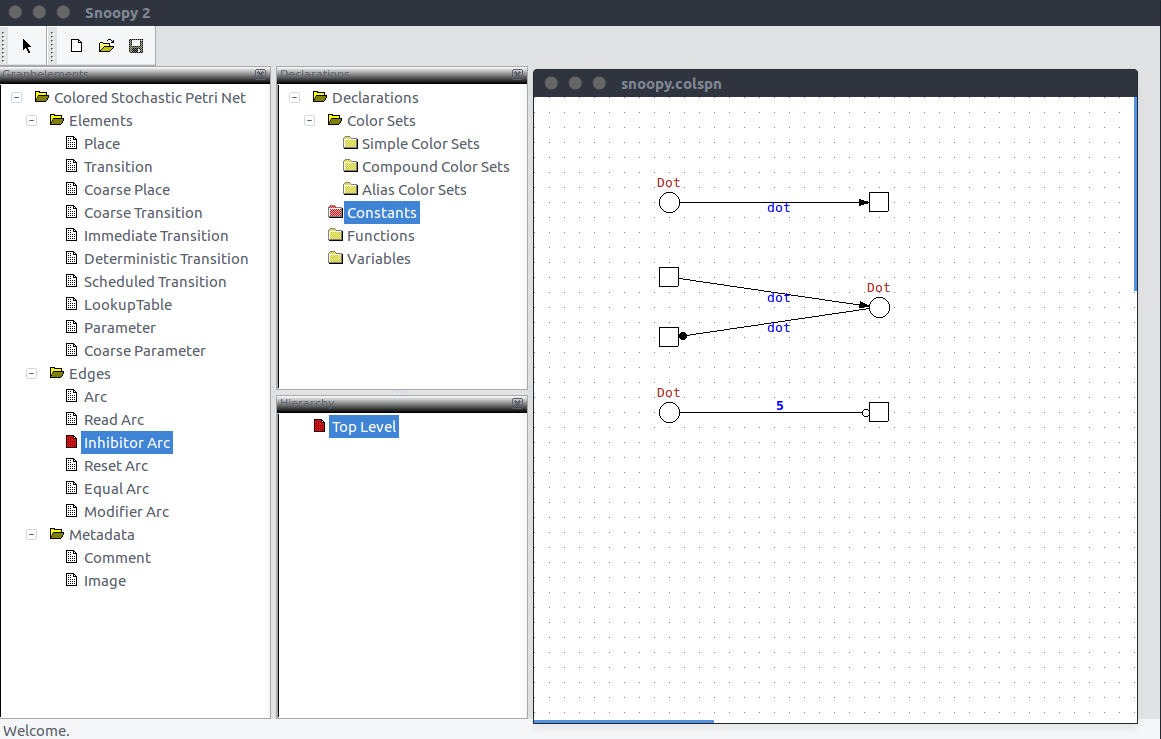
\includegraphics[scale=0.3]{imagens/snoopy.png}
				\caption{Captura de tela da ferramenta Snoopy}
			\end{center}
		\end{figure}

	\section{Modelo - Interação bactéria-neutrófilo}\label{Bacteria-NeutrophilModel}
	
		Durante o desenvolvimento deste trabalho, foram construídas várias redes de Petri
		estocásticas que modelam processos e interações que ocorrem durante a resposta imune inata a uma
		infecção bacteriana. O objetivo inicial foi construir uma rede simples que conseguisse capturar dois
		comportamentos: 
		
		\begin{description}
			\item[Eliminação das bactérias] Cenário onde os neutrófilos conseguem, durante o tempo simulado, 
			eliminar completamente as bactérias.
			\item[Infecção persistente] Cenário onde os neutrófilos já não são capazes de eliminar as bactérias 
			que persistem no hospedeiro, podendo inclusive apresentar uma tendência de crescimento com o passar do tempo.
		\end{description}
		
		A rede de Petri mais simples construída que é capaz de exibir esses dois comportamentos é mostrada na Figura \ref{fig:primeiraRede}. 
	
		\begin{figure}
			\begin{center}
				\begin{tikzpicture}[x=0.5pt,y=-0.5pt]

\definecolor{BLACK}{RGB}{0,0,0}
\definecolor{r232g19b19}{RGB}{232,19,19}
\draw[BLACK, solid, line join=round, line cap=round, line width=1, fill=r232g19b19]
	(199,143) ellipse[x radius=10, y radius=10];
\draw[BLACK]
	(179,158.5) node[rotate=0, font=\ttfamily\normalsize, BLACK, right=-.25]
	{B};
\draw[BLACK]
	(191,141.5) node[rotate=0, font=\ttfamily\normalsize, BLACK, right=-.25]
	{10};
\definecolor{RED}{RGB}{255,0,0}
\draw[BLACK]
	(180,123.5) node[rotate=0, font=\ttfamily\normalsize, RED, right=-.25]
	{10`dot};
\definecolor{r18g244b21}{RGB}{18,244,21}
\draw[BLACK, solid, line join=round, line cap=round, line width=1, fill=r18g244b21]
	(430,144) ellipse[x radius=10, y radius=10];
\draw[BLACK]
	(447,143.5) node[rotate=0, font=\ttfamily\normalsize, BLACK, right=-.25]
	{N};
\definecolor{WHITE}{RGB}{255,255,255}
\draw[BLACK, solid, line join=round, line cap=round, line width=1, fill=WHITE]
	(50,133) rectangle +(20,20);
\draw[BLACK]
	(43,117.5) node[rotate=0, font=\ttfamily\normalsize, BLACK, right=-.25]
	{B\_Replication};
\draw[BLACK, solid, line join=round, line cap=round, line width=1, fill=WHITE]
	(291,133) rectangle +(20,20);
\draw[BLACK]
	(250,162.5) node[rotate=0, font=\ttfamily\normalsize, BLACK, right=-.25]
	{Phagocytosis};
\draw[BLACK, solid, line join=round, line cap=round, line width=1, fill=WHITE]
	(420,251) rectangle +(20,20);
\draw[BLACK]
	(174,283.5) node[rotate=0, font=\ttfamily\normalsize, BLACK, right=-.25]
	{Neutrophil\_Death\_Caused\_by\_the\_Bacteria};
\draw[BLACK, solid, line join=round, line cap=round, line width=1, fill=WHITE]
	(420,30) rectangle +(20,20);
\draw[BLACK]
	(399,20.5) node[rotate=0, font=\ttfamily\normalsize, BLACK, right=-.25]
	{N\_Migration};
\draw[BLACK, solid, line join=round, line cap=round, line width=1]
	(70,143) -- (189,143);
\draw[BLACK, solid, line join=round, line cap=round, line width=1, fill=BLACK]
	(189,143) -- (179,146) -- (179,140) -- (189,143) -- cycle;
\draw[BLACK, solid, line join=round, line cap=round, line width=1]
	(209,143) -- (291,143);
\draw[BLACK, solid, line join=round, line cap=round, line width=1, fill=BLACK]
	(291,143) -- (281,146) -- (281,140) -- (291,143) -- cycle;
\draw[BLACK, solid, line join=round, line cap=round, line width=1]
	(430,154) -- (430,251);
\draw[BLACK, solid, line join=round, line cap=round, line width=1, fill=BLACK]
	(430,251) -- (427,241) -- (433,241) -- (430,251) -- cycle;
\draw[BLACK, solid, line join=round, line cap=round, line width=1]
	(430,50) -- (430,134);
\draw[BLACK, solid, line join=round, line cap=round, line width=1, fill=BLACK]
	(430,134) -- (427,124) -- (433,124) -- (430,134) -- cycle;
\draw[BLACK, solid, line join=round, line cap=round, line width=1]
	(189,143) -- (70,143);
\draw[BLACK, solid, line join=round, line cap=round, line width=1, fill=BLACK]
	(73.5,143.5) ellipse[x radius=3.5, y radius=3.5];
\draw[BLACK, solid, line join=round, line cap=round, line width=1]
	(200,153) -- (205,206.5) .. controls (210,260) .. (315,260.5) -- (420,261);
\draw[BLACK, solid, line join=round, line cap=round, line width=1, fill=BLACK]
	(416.5,260.5) ellipse[x radius=3.5, y radius=3.5];
\draw[BLACK, solid, line join=round, line cap=round, line width=1]
	(200,133) -- (205,86.5) .. controls (210,40) .. (315,40) -- (420,40);
\draw[BLACK, solid, line join=round, line cap=round, line width=1, fill=BLACK]
	(416.5,40.5) ellipse[x radius=3.5, y radius=3.5];
\draw[BLACK, solid, line join=round, line cap=round, line width=1]
	(311,139) -- (336,129.5) .. controls (361,120) .. (390.5,130.5) -- (420,141);
\draw[BLACK, solid, line join=round, line cap=round, line width=1, fill=BLACK]
	(420,141) -- (409,140) -- (412,134) -- (420,141) -- cycle;
\draw[BLACK, solid, line join=round, line cap=round, line width=1]
	(420,146) -- (391,153) .. controls (362,160) .. (336.5,153) -- (311,146);
\draw[BLACK, solid, line join=round, line cap=round, line width=1, fill=BLACK]
	(314.5,146.5) ellipse[x radius=3.5, y radius=3.5];
\end{tikzpicture}
			\end{center}
			\caption{Rede mais simples que representa a interação bactéria-neutrófilo}
			\label{fig:primeiraRede}
		\end{figure}

		Essa rede de Petri possui dois places: \textbf{B} (que representa as bactérias) e \textbf{N} (que representa os
		neutrófilos). A rede possui um único colorset (o colorset \textit{Dot}) que é o mesmo usado em redes de Petri não
		coloridas. O tipo de dados dot representa um token que pode ser transmitido entre \textit{places} e transições.
		O \textit{place} B começa com um marking inicial de 10 dots representando uma infecção inicial do tecido e o
		\textit{place} N começa com 0 dots representando o fato de que inicialmente, na ausência de infecção, não há
		neutrófilos no tecido.
		
		Os seguintes processos foram modelados com essa rede:
		
		\begin{enumerate}
		  \item Replicação (transição Replication): as bactérias se replicam com uma probabilidade dada por
		  $\frac{0.1 B}{B + 1}$. Essa função modela uma replicação com saturação, onde a probabilidade de
		  replicação aumenta lentamente com a quantidade de bactérias até saturar em 0.1. Essa
		  saturação é necessária para evitar uma replicação exponencial das bactérias. Para modelar a
		  replicação, foi utilizado um arco de leitura (arco Read) como arco de entrada e um arco padrão
		  como arco de saída. Essa escolha se deve ao fato de que um arco de leitura pode alterar a taxa
		  de disparo de uma transição não consumindo os tokens dos pré-places como explicado na
		  Seção \ref{Arcos}. 
		  \item Fagocitose (transição Phagocytosis): uma bactéria é fagocitada quando encontra um neutrófilo.
		  Nesse caso, a bactéria perde um token e a quantidade de tokens do neutrófilo fica inalterada.
		  Essa transição ocorre com probabilidade $\frac{0.01 B N}{0.5 B + 1}$. Essa função modela o fato de que
		  a probabilidade de fagocitose é proporcional ao número de bactérias e neutrófilos, ou seja,
		  quanto maior o número de bactérias e/ou de neutrófilos maior é o valor da função. A função
		  também possui uma saturação dependente da quantidade de bactérias. Nesse caso, o termo
		  $0.5 B + 1$ no denominador modela uma diminuição na probabilidade da transição ocorrer à
		  medida que a quantidade de bactérias aumenta e seu uso é motivado por mecanismos
		  empregados pela bactéria para escapar da fagocitose.
		  \item Migração dos neutrófilos (transição Neutrophil\_Migration): A migração dos neutrófilos para o tecido 
		  ocorre quando há uma infecção. A função de transição é dada por $\frac{0.1 B}{B + 1}$. Nesse caso, a probabilidade 
		  de migração aumenta com a quantidade de bactérias e também há uma inibição desse processo realizada 
		  pela própria bactéria. Essa inibição também é motivada por mecanismos biológicos empregados pela bactéria 
		  que atrapalham a migração de células do sistema imune para o tecido infectado. 
		  \item Morte dos neutrófilos (transição Neutrophil\_Death\_Caused\_by\_the\_Bacteria): As bactérias produzem 
		  diversas toxinas (não modeladas explicitamente na rede) que causam a morte dos neutrófilos. 
		  A morte dos neutrófilos é proporcional à concentração de bactérias e de neutrófilos e é modelada pela 
		  função $0.001 B N$. 
		\end{enumerate}
		
	\section[Modelo com Dano Tecidual]{Modelo com Dano Tecidual}
	
	%%%TODO Citar dissertação Alexandre e artigo BMC
		Com o objetivo de estudar infecções crônicas e seus efeitos na resposta imune inata, foi desenvolvida uma 
		outra rede de Petri (Figura \ref{fig:redeDano}) que modela novas populações e novos processos. 
		As novas populações modeladas são: macrófagos (\textit{place} Macrophages), macrófagos mortos (\textit{place} MD), o dano tecidual (\textit{place} Damage), 
		neutrófilos apoptóticos (\textit{place} $ND$) e citocinas anti-inflamatórias (\textit{place} $AC$).
		
% 		Vários processos presentes nas respostas imunes são considerados como, por exemplo: iniciação da resposta imune pelos macrófagos atraindo neutrófilos para o local 
% 		da infecção, fagocitose da bactéria realizada pelos macrófagos e neutrófilos, apoptose das células, morte dos neutrófilos causada pela bactéria (através 
% 		de toxinas e outros fatores que não são modelados explicitamente), fagocitose de células mortas realizada pelos macrófagos, dano tecidual causado pelas 
% 		bactérias e pelos neutrófilos necrosados, migração devido a inflamação, entre outros. 
		
		\begin{figure}
			\begin{center}
				\resizebox{\textwidth}{!}{
\begin{tikzpicture}[x=1pt,y=-1pt]
\definecolor{r255g3b0}{RGB}{255,3,0}
\definecolor{WHITE}{RGB}{255,255,255}
\draw[r255g3b0, solid, line join=round, line cap=round, line width=1, fill=WHITE]
	(590,870) ellipse[x radius=23, y radius=23];
\definecolor{BLACK}{RGB}{0,0,0}
\draw[BLACK]
	(586,868.5) node[rotate=0, font=\ttfamily\huge, BLACK, right=-.25]
	{B};
\definecolor{r0g16b200}{RGB}{0,16,200}
\draw[r0g16b200, solid, line join=round, line cap=round, line width=1, fill=WHITE]
	(960,470) ellipse[x radius=23, y radius=23];
\draw[BLACK]
	(958,468.5) node[rotate=0, font=\ttfamily\huge, BLACK, right=-.25]
	{N};
\definecolor{r99g94b94}{RGB}{99,94,94}
\draw[r99g94b94, solid, line join=round, line cap=round, line width=1, fill=WHITE]
	(590,680) ellipse[x radius=16, y radius=16];
\draw[BLACK]
	(586,684.5) node[rotate=0, font=\ttfamily\huge, BLACK, right=-.25]
	{D};
\definecolor{r219g204b0}{RGB}{219,204,0}
\draw[r219g204b0, solid, line join=round, line cap=round, line width=1, fill=WHITE]
	(960,290) ellipse[x radius=16, y radius=16];
\draw[BLACK]
	(949,288.5) node[rotate=0, font=\ttfamily\huge, BLACK, right=-.25]
	{ND};
\definecolor{r0g174b51}{RGB}{0,174,51}
\draw[r0g174b51, solid, line join=round, line cap=round, line width=1, fill=WHITE]
	(150,410) ellipse[x radius=29, y radius=29];
\draw[BLACK]
	(139,408.5) node[rotate=0, font=\ttfamily\huge, BLACK, right=-.25]
	{M};
\draw[BLACK, solid, line join=round, line cap=round, line width=1, fill=WHITE]
	(370,330) ellipse[x radius=12, y radius=12];
\draw[BLACK]
	(355,305.5) node[rotate=0, font=\ttfamily\huge, BLACK, right=-.25]
	{MD};
\definecolor{r255g0b183}{RGB}{255,0,183}
\draw[r255g0b183, solid, line join=round, line cap=round, line width=1, fill=WHITE]
	(840,1010) ellipse[x radius=17, y radius=17];
\draw[BLACK]
	(833,1008.5) node[rotate=0, font=\ttfamily\huge, BLACK, right=-.25]
	{AC};
\draw[BLACK, solid, line join=round, line cap=round, line width=1, fill=WHITE]
	(910,1120) ellipse[x radius=10, y radius=10];
\draw[BLACK]
	(890,1142.5) node[rotate=0, font=\ttfamily\huge, BLACK, right=-.25]
	{AC\_Aux};
\draw[BLACK, solid, line join=round, line cap=round, line width=1, fill=WHITE]
	(470,930) rectangle +(20,20);
\draw[BLACK]
	(425,958.5) node[rotate=0, font=\ttfamily\huge, BLACK, right=-.25]
	{Replication};
\draw[BLACK, solid, line join=round, line cap=round, line width=1, fill=WHITE]
	(740,671) rectangle +(20,18);
\draw[BLACK]
	(684,704.5) node[rotate=0, font=\ttfamily\huge, BLACK, right=-.25]
	{Phag\_B\_N};
\draw[BLACK, solid, line join=round, line cap=round, line width=1, fill=WHITE]
	(1081,460) rectangle +(18,20);
\draw[BLACK]
	(989,444.5) node[rotate=0, font=\ttfamily\huge, BLACK, right=-.25]
	{N\_Death\_Caused\_by\_B};
\draw[BLACK, solid, line join=round, line cap=round, line width=1, fill=WHITE]
	(580,560) rectangle +(20,20);
\draw[BLACK]
	(602,570.5) node[rotate=0, font=\ttfamily\huge, BLACK, right=-.25]
	{N\_Damage};
\draw[BLACK, solid, line join=round, line cap=round, line width=1, fill=WHITE]
	(580,750) rectangle +(20,20);
\draw[BLACK]
	(493,753.5) node[rotate=0, font=\ttfamily\bfseries\huge, BLACK, right=-.25]
	{B\_Damage};
\draw[BLACK, solid, line join=round, line cap=round, line width=1, fill=WHITE]
	(140,670) rectangle +(20,20);
\draw[BLACK]
	(107,702.5) node[rotate=0, font=\ttfamily\huge, BLACK, right=-.25]
	{Phag\_D\_M};
\draw[BLACK, solid, line join=round, line cap=round, line width=1, fill=WHITE]
	(300,560) rectangle +(20,20);
\draw[BLACK]
	(301,545.5) node[rotate=0, font=\ttfamily\huge, BLACK, right=-.25]
	{Phag\_B\_M};
\draw[BLACK, solid, line join=round, line cap=round, line width=1, fill=WHITE]
	(950,369) rectangle +(20,20);
\draw[BLACK]
	(847,356.5) node[rotate=0, font=\ttfamily\huge, BLACK, right=-.25]
	{Neutrophil\_Apoptosis};
\draw[BLACK, solid, line join=round, line cap=round, line width=1, fill=WHITE]
	(250,322) rectangle +(20,16);
\draw[BLACK]
	(215,305.5) node[rotate=0, font=\ttfamily\huge, BLACK, right=-.25]
	{M\_Apoptosis};
\draw[BLACK, solid, line join=round, line cap=round, line width=1, fill=WHITE]
	(951,859) rectangle +(18,22);
\draw[BLACK]
	(972,866.5) node[rotate=0, font=\ttfamily\huge, BLACK, right=-.25]
	{N\_Migration1};
\draw[BLACK, solid, line join=round, line cap=round, line width=1, fill=WHITE]
	(290,861) rectangle +(20,18);
\draw[BLACK]
	(193,855.5) node[rotate=0, font=\ttfamily\huge, BLACK, right=-.25]
	{M\_Migration1};
\draw[BLACK, solid, line join=round, line cap=round, line width=1, fill=WHITE]
	(950,220) rectangle +(20,20);
\draw[BLACK]
	(927,208.5) node[rotate=0, font=\ttfamily\huge, BLACK, right=-.25]
	{Phag\_ND\_M};
\draw[BLACK, solid, line join=round, line cap=round, line width=1, fill=WHITE]
	(770,1060) rectangle +(20,20);
\draw[BLACK]
	(687,1069.5) node[rotate=0, font=\ttfamily\huge, BLACK, right=-.25]
	{AC\_Decay};
\draw[BLACK, solid, line join=round, line cap=round, line width=1, fill=WHITE]
	(830,400) rectangle +(20,20);
\draw[BLACK]
	(733,388.5) node[rotate=0, font=\ttfamily\huge, BLACK, right=-.25]
	{M\_Migration2};
\draw[BLACK, solid, line join=round, line cap=round, line width=1, fill=WHITE]
	(390,460) rectangle +(20,20);
\draw[BLACK]
	(345,443.5) node[rotate=0, font=\ttfamily\huge, BLACK, right=-.25]
	{Inflammation\_Migration};
\draw[BLACK, solid, line join=round, line cap=round, line width=1, fill=WHITE]
	(900,1060) rectangle +(20,20);
\draw[BLACK]
	(927,1066.5) node[rotate=0, font=\ttfamily\huge, BLACK, right=-.25]
	{AC\_Prod};
\draw[BLACK, solid, line join=round, line cap=round, line width=1]
	(490,930) -- (505,915) .. controls (520,900) .. (543.5,890) -- (567,880);
\draw[BLACK, solid, line join=round, line cap=round, line width=1, fill=BLACK]
	(567,880) -- (559,887) -- (556,881) -- (567,880) -- cycle;
\draw[BLACK, solid, line join=round, line cap=round, line width=1]
	(609,847) -- (742,689);
\draw[BLACK, solid, line join=round, line cap=round, line width=1, fill=BLACK]
	(742,689) -- (739,699) -- (733,695) -- (742,689) -- cycle;
\draw[BLACK, solid, line join=round, line cap=round, line width=1]
	(983,470) -- (1081,470);
\draw[BLACK, solid, line join=round, line cap=round, line width=1, fill=BLACK]
	(1081,470) -- (1071,473) -- (1071,467) -- (1081,470) -- cycle;
\draw[BLACK, solid, line join=round, line cap=round, line width=1]
	(1083,460) -- (972,306);
\draw[BLACK, solid, line join=round, line cap=round, line width=1, fill=BLACK]
	(972,306) -- (980,312) -- (975,316) -- (972,306) -- cycle;
\draw[BLACK, solid, line join=round, line cap=round, line width=1]
	(590,580) -- (590,664);
\draw[BLACK, solid, line join=round, line cap=round, line width=1, fill=BLACK]
	(590,664) -- (587,654) -- (593,654) -- (590,664) -- cycle;
\draw[BLACK, solid, line join=round, line cap=round, line width=1]
	(590,750) -- (590,696);
\draw[BLACK, solid, line join=round, line cap=round, line width=1, fill=BLACK]
	(590,696) -- (593,706) -- (587,706) -- (590,696) -- cycle;
\draw[BLACK, solid, line join=round, line cap=round, line width=1]
	(574,680) -- (160,680);
\draw[BLACK, solid, line join=round, line cap=round, line width=1, fill=BLACK]
	(160,680) -- (170,677) -- (170,683) -- (160,680) -- cycle;
\draw[BLACK, solid, line join=round, line cap=round, line width=1]
	(567,866) -- (548.5,863) .. controls (530,860) .. (475,840) .. controls (420,820) .. (395,775) .. controls (370,730) .. (342,655) -- (314,580);
\draw[BLACK, solid, line join=round, line cap=round, line width=1, fill=BLACK]
	(314,580) -- (320,588) -- (314,591) -- (314,580) -- cycle;
\draw[BLACK, solid, line join=round, line cap=round, line width=1]
	(960,447) -- (960,389);
\draw[BLACK, solid, line join=round, line cap=round, line width=1, fill=BLACK]
	(960,389) -- (963,399) -- (957,399) -- (960,389) -- cycle;
\draw[BLACK, solid, line join=round, line cap=round, line width=1]
	(960,369) -- (960,306);
\draw[BLACK, solid, line join=round, line cap=round, line width=1, fill=BLACK]
	(960,306) -- (963,316) -- (957,316) -- (960,306) -- cycle;
\draw[BLACK, solid, line join=round, line cap=round, line width=1]
	(179,389) -- (250,337);
\draw[BLACK, solid, line join=round, line cap=round, line width=1, fill=BLACK]
	(250,337) -- (244,346) -- (240,340) -- (250,337) -- cycle;
\draw[BLACK, solid, line join=round, line cap=round, line width=1]
	(270,330) -- (358,330);
\draw[BLACK, solid, line join=round, line cap=round, line width=1, fill=BLACK]
	(358,330) -- (348,333) -- (348,327) -- (358,330) -- cycle;
\draw[BLACK, solid, line join=round, line cap=round, line width=1]
	(960,859) -- (960,493);
\draw[BLACK, solid, line join=round, line cap=round, line width=1, fill=BLACK]
	(960,493) -- (963,503) -- (957,503) -- (960,493) -- cycle;
\draw[BLACK, solid, line join=round, line cap=round, line width=1]
	(297,861) -- (159,439);
\draw[BLACK, solid, line join=round, line cap=round, line width=1, fill=BLACK]
	(159,439) -- (166,447) -- (159,450) -- (159,439) -- cycle;
\draw[BLACK, solid, line join=round, line cap=round, line width=1]
	(960,274) -- (960,240);
\draw[BLACK, solid, line join=round, line cap=round, line width=1, fill=BLACK]
	(960,240) -- (963,250) -- (957,250) -- (960,240) -- cycle;
\draw[BLACK, solid, line join=round, line cap=round, line width=1]
	(823,1027) -- (790,1060);
\draw[BLACK, solid, line join=round, line cap=round, line width=1, fill=BLACK]
	(790,1060) -- (795,1051) -- (799,1055) -- (790,1060) -- cycle;
\draw[BLACK, solid, line join=round, line cap=round, line width=1]
	(830,410) -- (179,410);
\draw[BLACK, solid, line join=round, line cap=round, line width=1, fill=BLACK]
	(179,410) -- (189,407) -- (189,413) -- (179,410) -- cycle;
\draw[BLACK, solid, line join=round, line cap=round, line width=1]
	(410,470) -- (937,470);
\draw[BLACK, solid, line join=round, line cap=round, line width=1, fill=BLACK]
	(937,470) -- (927,473) -- (927,467) -- (937,470) -- cycle;
\draw[BLACK, solid, line join=round, line cap=round, line width=1]
	(390,468) -- (179,417);
\draw[BLACK, solid, line join=round, line cap=round, line width=1, fill=BLACK]
	(179,417) -- (190,416) -- (188,423) -- (179,417) -- cycle;
\draw[BLACK, solid, line join=round, line cap=round, line width=1]
	(900,1061) -- (857,1025);
\draw[BLACK, solid, line join=round, line cap=round, line width=1, fill=BLACK]
	(857,1025) -- (867,1029) -- (862,1034) -- (857,1025) -- cycle;
\draw[BLACK, solid, line join=round, line cap=round, line width=1]
	(910,1110) -- (910,1080);
\draw[BLACK, solid, line join=round, line cap=round, line width=1, fill=BLACK]
	(910,1080) -- (913,1090) -- (907,1090) -- (910,1080) -- cycle;
\draw[BLACK, solid, line join=round, line cap=round, line width=1]
	(150,690) -- (150,870) .. controls (150,1050) .. (150,1085) .. controls (150,1120) .. (190,1120) .. controls (230,1120) .. (565,1120) -- (900,1120);
\draw[BLACK, solid, line join=round, line cap=round, line width=1, fill=BLACK]
	(900,1120) -- (890,1123) -- (890,1117) -- (900,1120) -- cycle;
\draw[BLACK, solid, line join=round, line cap=round, line width=1]
	(970,230) -- (1045,230) .. controls (1120,230) .. (1145,230) .. controls (1170,230) .. (1170,255) .. controls (1170,280) .. (1170,675) .. controls (1170,1070) .. (1170,1095) .. controls (1170,1120) .. (1150,1120) .. controls (1130,1120) .. (1025,1120) -- (920,1120);
\draw[BLACK, solid, line join=round, line cap=round, line width=1, fill=BLACK]
	(920,1120) -- (930,1117) -- (930,1123) -- (920,1120) -- cycle;
\draw[BLACK, solid, line join=round, line cap=round, line width=1]
	(567,893) -- (553.5,906.5) .. controls (540,920) .. (515,928.5) -- (490,937);
\draw[BLACK, solid, line join=round, line cap=round, line width=1, fill=BLACK]
	(493.5,935.5) ellipse[x radius=3.5, y radius=3.5];
\draw[BLACK, solid, line join=round, line cap=round, line width=1]
	(937,493) -- (759,671);
\draw[BLACK, solid, line join=round, line cap=round, line width=1, fill=BLACK]
	(761.5,668.5) ellipse[x radius=3.5, y radius=3.5];
\draw[BLACK, solid, line join=round, line cap=round, line width=1]
	(613,866) -- (691.5,853) .. controls (770,840) .. (860,805) .. controls (950,770) .. (1005,705) .. controls (1060,640) .. (1074,560) -- (1088,480);
\draw[BLACK, solid, line join=round, line cap=round, line width=1, fill=BLACK]
	(1087.5,483.5) ellipse[x radius=3.5, y radius=3.5];
\draw[BLACK, solid, line join=round, line cap=round, line width=1]
	(590,847) -- (590,770);
\draw[BLACK, solid, line join=round, line cap=round, line width=1, fill=BLACK]
	(590.5,773.5) ellipse[x radius=3.5, y radius=3.5];
\draw[BLACK, solid, line join=round, line cap=round, line width=1]
	(150,439) -- (150,670);
\draw[BLACK, solid, line join=round, line cap=round, line width=1, fill=BLACK]
	(150.5,666.5) ellipse[x radius=3.5, y radius=3.5];
\draw[BLACK, solid, line join=round, line cap=round, line width=1]
	(179,439) -- (300,560);
\draw[BLACK, solid, line join=round, line cap=round, line width=1, fill=BLACK]
	(297.5,557.5) ellipse[x radius=3.5, y radius=3.5];
\draw[BLACK, solid, line join=round, line cap=round, line width=1]
	(613,870) -- (951,870);
\draw[BLACK, solid, line join=round, line cap=round, line width=1, fill=BLACK]
	(947.5,870.5) ellipse[x radius=3.5, y radius=3.5];
\draw[BLACK, solid, line join=round, line cap=round, line width=1]
	(567,870) -- (458.5,870) .. controls (350,870) .. (330,870) -- (310,870);
\draw[BLACK, solid, line join=round, line cap=round, line width=1, fill=BLACK]
	(313.5,870.5) ellipse[x radius=3.5, y radius=3.5];
\draw[BLACK, solid, line join=round, line cap=round, line width=1]
	(944,290) -- (812,290) .. controls (680,290) .. (635,290) .. controls (590,290) .. (590,325) .. controls (590,360) .. (590,460) -- (590,560);
\draw[BLACK, solid, line join=round, line cap=round, line width=1, fill=BLACK]
	(590.5,556.5) ellipse[x radius=3.5, y radius=3.5];
\draw[BLACK, solid, line join=round, line cap=round, line width=1]
	(150,381) -- (150,345.5) .. controls (150,310) .. (150,270) .. controls (150,230) .. (190,230) .. controls (230,230) .. (590,230) -- (950,230);
\draw[BLACK, solid, line join=round, line cap=round, line width=1, fill=BLACK]
	(946.5,230.5) ellipse[x radius=3.5, y radius=3.5];
\draw[BLACK, solid, line join=round, line cap=round, line width=1]
	(937,459) -- (850,415);
\draw[BLACK, solid, line join=round, line cap=round, line width=1, fill=BLACK]
	(853.5,416.5) ellipse[x radius=3.5, y radius=3.5];
\draw[BLACK, solid, line join=round, line cap=round, line width=1]
	(576,664) -- (409,480);
\draw[BLACK, solid, line join=round, line cap=round, line width=1, fill=BLACK]
	(411.5,482.5) ellipse[x radius=3.5, y radius=3.5];
\draw[BLACK, loosely dashed, line join=round, line cap=round, line width=1]
	(574,674) -- (320,574);
\draw[BLACK, solid, line join=round, line cap=round, line width=1, fill=BLACK]
	(320,574) -- (331,574) -- (328,581) -- (320,574) -- cycle;
\draw[BLACK, loosely dashed, line join=round, line cap=round, line width=1]
	(857,1010) -- (888.5,1010) .. controls (920,1010) .. (940,1010) .. controls (960,1010) .. (960,990) .. controls (960,970) .. (960,925.5) -- (960,881);
\draw[BLACK, solid, line join=round, line cap=round, line width=1, fill=BLACK]
	(960,881) -- (963,891) -- (957,891) -- (960,881) -- cycle;
\draw[BLACK, loosely dashed, line join=round, line cap=round, line width=1]
	(606,680) -- (740,680);
\draw[BLACK, solid, line join=round, line cap=round, line width=1, fill=BLACK]
	(740,680) -- (730,683) -- (730,677) -- (740,680) -- cycle;
\draw[BLACK, loosely dashed, line join=round, line cap=round, line width=1]
	(840,993) -- (840,420);
\draw[BLACK, solid, line join=round, line cap=round, line width=1, fill=BLACK]
	(840,420) -- (843,430) -- (837,430) -- (840,420) -- cycle;
\draw[BLACK, loosely dashed, line join=round, line cap=round, line width=1]
	(823,1010) -- (591.5,1010) .. controls (360,1010) .. (330,1010) .. controls (300,1010) .. (300,985) .. controls (300,960) .. (300,919.5) -- (300,879);
\draw[BLACK, solid, line join=round, line cap=round, line width=1, fill=BLACK]
	(300,879) -- (303,889) -- (297,889) -- (300,879) -- cycle;
\draw[BLACK, loosely dashed, line join=round, line cap=round, line width=1]
	(839,993) -- (829.5,806.5) .. controls (820,620) .. (795,575) .. controls (770,530) .. (715,510) .. controls (660,490) .. (535,480.5) -- (410,471);
\draw[BLACK, solid, line join=round, line cap=round, line width=1, fill=BLACK]
	(410,471) -- (420,468) -- (420,475) -- (410,471) -- cycle;
\end{tikzpicture}
}


			\end{center}
			\caption{Rede de Petri para a resposta imune inata considerando o papel regulador dos macrófagos e os efeitos do dano tecidual. 
			As bactérias são representadas pelo \textit{place} Bacteria na cor vermelha, os neutrófilos são representados pelo \textit{place} Neutrophil em azul, 
			os neutrófilos apoptóticos são representados pelo \textit{place} ND em amarelo, os macrófagos são representados pelo \textit{place} Macrophages 
			em verde, macrófagos mortos são representados pelo \textit{place} MD na cor preta, 
			o dano tecidual é representado pelo \textit{place} Damage em cinza e as citocinas anti-inflamatórias são representadas pelo \textit{place} 
			AC na cor rosa. As transições são representadas pelos quadrados. }
			\label{fig:redeDano}
		\end{figure}
		
		%- Justificar a escolha do macrófago e do dano tecidual:
		Os macrófagos foram escolhidos por desempenharem um papel muito importante na regulação da resposta imune, 
		controlando a inflamação e limpando o local da infecção através da fagocitose dos neutrófilos apoptóticos (transição Phag\_ND\_M), 
		da fagocitose de células de tecido mortas (transição Phag\_D\_M) e da produção de citocinas anti-inflamatórias (produção de AC). 
		A fagocitose dos neutrófilos apoptóticos é importante para evitar que os neutrófilos sofram necrose e liberem, como consequência desse processo, 
		um conjunto de substâncias que podem causar dano tecidual. Outro processo importante, a fagocitose de células mortas, evita mais inflamação e 
		mais dano tecidual. As citocinas anti-inflamatórias são responsáveis por regular a entrada de novas células do sistema imune (principalmente 
		neutrófilos) no local da infecção, impedindo um crescimento da inflamação e dos danos teciduais.
		
		Jarrett \textit{et al.} \cite{Jarrett2015} acreditam que a resposta anti-inflamatória dos macrófagos e a via reguladora 
		da resposta adaptativa são importantes para o controle da inflamação, evitando mais danos aos tecidos, limpando e 
		liberando o local da infecção para que a resposta adaptativa pró-inflamatória funcione melhor no ambiente 
		em questão. Eles também destacam a importância das respostas Treg e Th2 \cite{Jarrett2015}. 
						
		A importância dos macrófagos também é destacada no trabalho de Cohen \textit{et al.} \cite{Cohen2016}. 
		A pneumonia bacteriana, como a causada por \textit{S. aureus}, é associada com um influxo de neutrófilos 
		no tecido do pulmão e nas vias respiratórias. A regulação e limpeza dos neutrófilos recrutados é essencial 
		para prevenir um dano tecidual causado pelo ``fogo amigo'', sendo essa uma responsabilidade dos macrófagos 
		em um processo chamado eferocitose. Cohen \textit{et al.} \cite{Cohen2016} hipotetizaram que a bactéria \textit{S. aureus} 
		prejudica a eferocitose realizada pelos macrófagos alveolares através da atividade do fator de 
		virulência chamado \textit{alpha toxin}, que também está associado com alterações na função antimicrobial 
		dos macrófagos alveolares.
		
		Nós acreditamos que uma possível explicação para essa importância pode estar também no fato de que, 
		no contexto de infecções persistentes com a bactéria \textit{S. aureus}, a presença de 
		quantidades consideráveis de neutrófilos necróticos, células de tecido mortas e outras células mortas 
		prejudica as interações entre neutrófilos e bactérias, entre células B plasmáticas e bactérias 
		assim como entre os anticorpos e as bactérias. 
		
		\subsection{Processos modelados}
						
		As transições que modelam os novos processos considerados na rede de Petri são descritas na tabela \ref{tab:tabletransitions}.
		Nessa tabela, apresentamos o nome da transição, uma breve descrição do processo modelado pela transição, os efeitos do processo, 
		os \textit{places} que participam da transição e com quais tipos de arcos estão ligados a ela, além de apresentar a função de transição utilizada. 
	
		%%%TODO Acrescentar transições Phag_ND_M e AC_Decay. Mudar a função de transição Neutrophil_Migration_2.
		%Destacar que as funções de transição da tabela se referem ao cenário da resposta imune normal. 
		\begingroup
	\renewcommand{\arraystretch}{1.5} % Default value: 1
	\begin{center}
		\def\arraystretch{2}
		\begin{longtable}{
				>{\centering\arraybackslash}m{2cm}|
				m{4.23cm}|
				>{\centering\arraybackslash}m{3cm}|
				m{3cm}|
				>{\centering\arraybackslash}m{2.5cm}
			}
			
			\caption{Transições}
			\label{tab:tabletransitions}\\
			
			\textbf{Nome} & \textbf{Descrição} & \textbf{Efeito} & \textbf{Places} & \textbf{Função}\\ \hline
			\endfirsthead
			
			\multicolumn{5}{c}{{\bfseries \tablename\ \thetable{} -- continuando da página anterior}} \\
			\textbf{Nome} & \textbf{Descrição} & \textbf{Efeito} & \textbf{Places} & \textbf{Função}\\
			\endhead
			
			\multicolumn{5}{r}{{Continua na próxima página}} \\
			\endfoot
			\hline \hline
			\endlastfoot
			
			Replication & 
			As bactérias se replicam com determinada probabilidade e a replicação possui uma saturação. & 
			Aumenta o número de tokens de B em 1. & 
			\parbox{3cm}{B [arc in = read, \\\ arc out = std]} & 
			$\frac{0.5 \times B}{B + 1}$ \\ \hline 
			
			Phag\_B\_N & 
			Modela a fagocitose das bactérias realizada pelos neutrófilos. & 
			Diminui o número de tokens de B em 1. & 
			\parbox{3cm}{B [arc in = std],\\\ N [arc in = read]\\\ D [arc in = mod]} & 			
			$\frac{0.1 \times B \times N}{0.5 \times B + 0.1 \times D + 1}$ \\ \hline
			
			Phag\_B\_M & 
			Modela a fagocitose das bactérias realizada pelos macrófagos.  & 
			Diminui o número de tokens de B em 1.  & 
			\parbox{3cm}{B [arc in = std]\\\ M [arc in = read]\\\ D [arc in = mod]} & 
			$\frac{0.05 \times B \times M}{0.5 \times B + 0.1 \times D + 1}$ \\ \hline
			
			
			N\_Death\_B & Modela a morte de neutrófilos causada pelas bactérias.  & 
			Diminui o número de tokens de N em 1.  & 
			\parbox{3cm}{B [arc in = read]\\\ N [arc in = std]\\\ ND [arc out = std]} & 
			$0.005 \times B \times N$ \\ \hline
			
			%M\_Death\_B & 
			%Modela a morte de macrófagos causada pelas bactérias.  & 
			%Diminui o número de tokens de M em 1.  & 
			%B [arc in = read] e M [arc in = std] & 
			%$0.0005 B M$ \\ \hline
			
			Inflam\_Mig & 
			Modela a migração de neutrófilos e macrófagos como consequência da inflamação causada pela morte de células do sistema imune e pelo dano tecidual.  & 
			Aumenta em 1 o número de tokens de N e M. & 
			\parbox{3cm}{D[arc in = read]\\\ AC[arc in = mod]\\\ N[arc out = std]\\\ M[arc out = std]} & 
			$0.005 \times D$ \\\hline
			
			N\_Migration1 & 
			Modela a migração dos neutrófilos atraídos pelas bactérias. 			
% 			devido a ação de citocinas pró-inflamatórias que não são modeladas explicitamente. 
% 			Essa transição simula a produção de citocinas pró-inflamatórias por outras células 
% 			(células de tecido e outras células do sistema imune não consideradas no modelo). 
			& 
			Aumenta o número de tokens de N em 1.  & 
			\parbox{3cm}{B[arc in = read]\\\ AC[arc in = mod] \\\ N [arc out = std] } & 
			$\frac{0.1 \times B}{0.1 \times B + 0.3 \times AC + 1}$ \\ \hline
						
% 			N\_Migration2 & 
% 			Modela a migração dos neutrófilos atraídos pelos macrófagos. & 
% 			Aumenta o número de tokens de N em 1.  & 
% 			\vspace{-0.41cm} \parbox{3cm}{B [arc in = read]\\\  N\_Mig2\_Aux \\\ [arc in = std]\\\ N [arc out = std]} \vspace{0cm} & 
% 			$\frac{0.05 N\_Mig2\_Aux}{(0.5 B + 1)}$ \\ \hline
			
			M\_Migration1 & 
			Modela a migração dos macrófagos atraídos pela bactéria. & 
			Aumenta em 1 o número de tokens de M. & 
			\parbox{3cm}{B[arc in = read]\\\ AC[arc in = mod]\\\ M[arc out = std]} & 
			$\frac{0.001 \times B + 0.000001}{0.1 \times AC + 1}$ \\\hline
			
			M\_Migration2 & 
			Modela a migração dos macrófagos atraídos pelos neutrófilos. & 
			Aumenta em 1 o número de tokens de M. & 
			\parbox{3cm}{N[arc in = read]\\\ AC[arc in = mod]\\\ M[arc out = std]} & 
			$\frac{0.001 \times N}{0.1 \times AC + 1}$ \\\hline
			
			N\_Apoptosis & 
			Modela a apoptose dos neutrófilos. & 
			Diminui em 1 o número de tokens de N. & 
			\parbox{3cm}{N [arc in = std]\\\ ND[arc out = std]} & 
			$0.02 \times N$ \\ \hline
			
			M\_Apoptosis & Modela a apoptose dos macrófagos. & 
			Diminui em 1 o número de tokens de M. & 
			\parbox{3cm}{M [arc in = std]\\\ MD [arc out = std]} & 
			$0.001 \times M$ \\	\hline
			
			B\_Damage & 
			Modela o dano tecidual causado pelas bactérias. & 
			Aumenta em 1 o número de tokens de D. & 
			\parbox{3cm}{B [arc in = read]\\\ D [arc out = std]} & 
			$0.005 \times B$ \\ \hline
			
			N\_Damage & 
			Modela o dano tecidual causado pelos neutrófilos necróticos. & 
			Aumenta em 1 o número de tokens de D. & 
			\parbox{3cm}{ND [arc in = read]\\\ D [arc out = std]} & 
			$0.01 \times ND$ \\ \hline
			
			Phag\_D\_M & 
			Modela a fagocitose de células de tecido mortas realizada pelos macrófagos. & 
			Diminui em 1 o número de tokens de D. & 
			\parbox{3cm}{D [arc in = std]\\\ M [arc in = read] \\\ AC\_Aux[arc out=std]} & 
			$0.005 \times M \times D$ \\ \hline
			
			Phag\_ND\_M & 
			Modela a fagocitose de neutrófilos apoptóticos realizada pelos macrófagos. & 
			Diminui em 1 o número de tokens de ND. & 
			\parbox{3cm}{ND [arc in = std]\\\ M [arc in = read] \\\ AC\_Aux[arc out=std]} & 
			0.05 $\times$ M $\times$ ND \\ \hline
			
			AC\_Prod & 
			Modela a produção de citocinas anti-inflamatórias. & 
			Aumenta em 1 o número de tokens de AC. & 
			\parbox{3cm}{AC\_Aux[arc in = std] \\\ AC[arc out=std]} & 
			$0.05 \times AC\_Aux$ \\\hline
			
			AC\_Decay & 
			Modela o decaimento de citocinas anti-inflamatórias. & 
			Diminui em 1 o número de tokens de AC. & 
			\parbox{3cm}{AC[arc in = std]} & 
			$0.05 \times AC$ \\
			
		\end{longtable}
	\end{center}
\endgroup


% \begin{sidewaystable}
%     \centering
% \caption{Wide table}
%     \label{tab:wide-item-tbl}
% \begin{tabularx}{\textwidth}{|*{4}{>{\RaggedRight\arraybackslash}X|}}
%     \hline
% \lipsum[1]  &   \lipsum[2]  &   \lipsum[3]  &   \lipsum[4]  \\
% \end{tabularx}
% \end{sidewaystable}

% \begin{longtable}{@{*}r||p{1in}@{*}}
% KILLED & LINE!!!! \kill
% \caption{Transições\label{long}}\\
% \hline\hline
% \multicolumn{2}{@{*}c@{*}}%
% {This part appears at the top of the table}\\
% \textsc{First}&\textsc{Second}\\
% \hline\hline
% \endfirsthead
% \caption[]{(continued)}\\
% \hline\hline
% \multicolumn{2}{@{*}c@{*}}%
% {This part appears at the top of every other page}\\
% \textbf{First}&\textbf{Second}\\
% \hline\hline
% \endhead
% \hline
% This goes at the&bottom.\\
% \hline
% \endfoot
% \hline
% These lines will&appear\\
% in place of the & usual foot\\
% at the end& of the table\\
% \hline
% \endlastfoot
% longtable  columns  are specified& in the \\
% same way as  in the tabular& environment.\\
% ...
% %\multicolumn{2}{||c||}{This is a ...}
% ...
% Some lines may take...&
% \raggedleft This last column is a ‘‘p’’ column...
% \tabularnewline
% ...
% Lots of lines& like this.\\
% ...
% \hline
% Lots\footnote{...} of lines& like this.\\
% Lots   of   lines& like this\footnote{...}\\
% \hline
% Lots of lines& like this.\\
% ...
% \end{longtable}

% \begin{tabulary}{\textwidth}{LCLLL}
%     \hline
%     \textbf{Name} & \textbf{Description} & \textbf{Effect} & \textbf{Places involved} & {Function}\\      
%     \hline    
%     Replication & As bactérias se replicam com determinada probabilidade e a replicação possui uma saturação. & Increase the number of tokens in B by 1.  & B [input arc = read, output arc = standard] & $\frac{0.1 B}{B + 1}$ \\
%     \hline
% \end{tabulary} 

		
		Analisando-se a tabela de transições, destaca-se as seguintes características do modelo:
		\begin{itemize}
		 \item O dano tecidual influência negativamente os processos de fagocitose. %Foi considerada essa hipótese a partir dos trabalhos de 
		 \item As citocinas anti-inflamatórias influenciam negativamente todos os processos de migração de neutrófilos e macrófagos 
		 que são modelados pelas transições N\_Migration1, M\_Migration1, M\_Migration2 e Inflammation\_Migration. Dessa forma, 
		 atuam na regulação da resposta imune contribuindo para a resolução da inflamação durante um processo infeccioso. 
		 \item A transição Inflammation\_Migration modela o recrutamento de mais células do sistema imune (neutrófilos e macrófagos) 
		 devido aos efeitos da inflamação (aumento do fluxo sanguíneo, aumento da permeabilidade do endotélio dos vasos, sinalização 
		 pró-inflamatória como consequência da morte de células, entre outros).
		 \item Através das transições Phag\_D\_M e Phag\_ND\_M, o macrófago realiza a limpeza do local infectado 
		 contribuindo para o término da inflamação. 
		 
		\end{itemize}

		
		%- *Destacar alguns dos novos processos considerados, explicando as interações entre os places. 		
		%- 		
		
		%É importante também destacar os processos que sofrem inibição da bactéria: 
	
	%\section{Difusão 1D}
	
	\section{Resultados}
	
		Para analisar as redes de Petri construídas e verificar os comportamentos que podem ser obtidos, realizou-se diversas simulações considerando-se 
		diferentes cenários. Os cenários simulados tentam refletir diferentes condições fisiológicas e patológicas encontradas na literatura assim como 
		tentam ilustrar o efeito de determinadas variáveis e processos na dinâmica do sistema. 
		Os resultados mostram a evolução do \textit{marking} dos \textit{places} ao longo do tempo. 
		%Podemos também observar o comportamento das transições ao longo do tempo.
	
		\subsection{Rede de Petri da interação bactéria-neutrófilo} 
		
		%%%
		%No caso da rede de Petri mais simples, foram simulados dois cenários:
		Para a rede de Petri que modela a interação bactéria-neutrófilo, foi simulado somente o cenário de uma 
		resposta imune ``normal'', ou seja, as taxas de migração e fagocitose foram ajustadas de forma que os 
		neutrófilos conseguissem eliminar as bactérias na maioria das simulações. 
		%não foi considerado nenhum mecanismo que prejudique os processos de fagocitose e migração dos neutrófilos. 
		
		Os resultados para o cenário da resposta imune ``normal'' podem ser observados nas Figuras \ref{redeSimples_fig2} 
		e \ref{redeSimples_fig1}.		
		
		\begin{figure}
			\begin{center}
				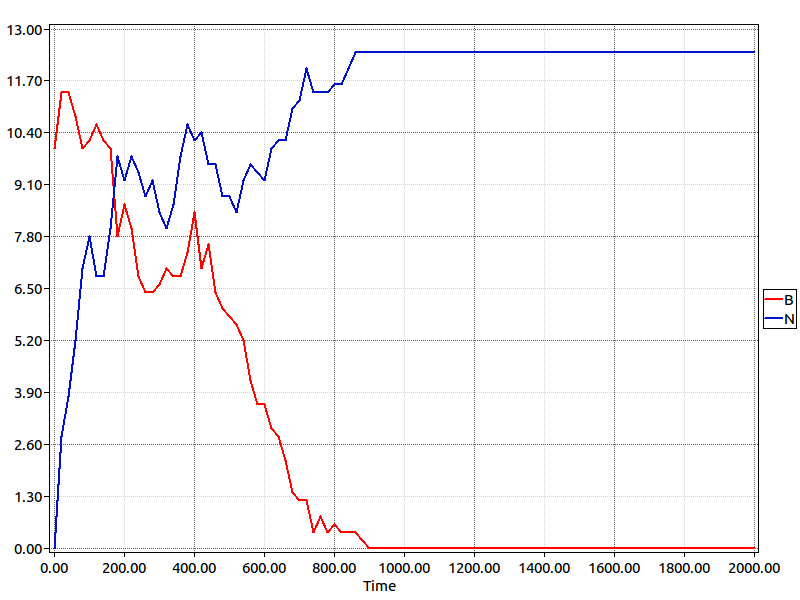
\includegraphics[scale=0.45]{imagens/resultados/RedesimplesB_N-fig2.png}
			\end{center}
			\caption{Eliminação da infecção obtida pela rede de Petri da interação bactéria-neutrófilo.  
			B representa as bactérias e N representa os neutrófilos.}
			\label{redeSimples_fig2}
		\end{figure}
		
		Na Figura \ref{redeSimples_fig2}, observa-se que as bactérias foram completamente eliminadas. 
		As bactérias iniciam com um \textit{marking} igual a 10 (tokens do tipo \textit{dot}) e os neutrófilos iniciam com um \textit{marking} igual a 0, ou seja, 
		a quantidade inicial de bactérias é 10 e a de neutrófilos é 0. 		
		Observa-se na Figura \ref{redeSimples_fig2} que as bactérias apresentam um crescimento pequeno no início e depois decrescem até serem eliminadas. 
		Esse decrescimento foi devido a fagocitose realizada por um maior número de neutrófilos que migraram para o tecido. Após a eliminação das bactérias, 
		a quantidade de neutrófilos se estabiliza devido ao fato de que não foi modelado o processo de apoptose ou morte natural dos neutrófilos. 		
		
		\begin{figure}
			\begin{center}
				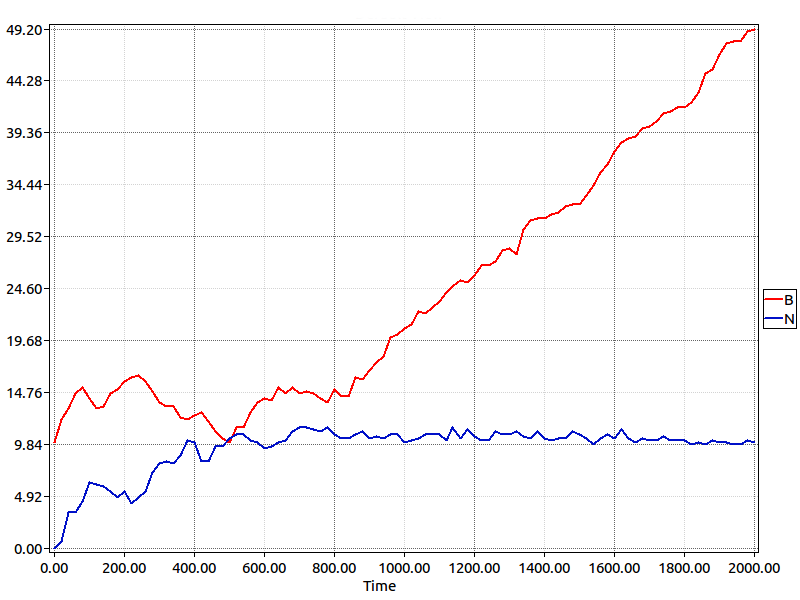
\includegraphics[scale=0.45]{imagens/resultados/RedesimplesB_N-fig1.png}
			\end{center}
			\caption{Infecção persistente obtida pela rede de Petri da interação bactéria-neutrófilo.  
			B representa as bactérias e N representa os neutrófilos. 
			}
			\label{redeSimples_fig1}
		\end{figure}
				
		Na Figura \ref{redeSimples_fig1}, observa-se que os neutrófilos não foram capazes de eliminar as bactérias. 
		Nesse caso, as bactérias foram bem sucedidas em persistir no hospedeiro. Esse cenário ilustra uma infecção crônica. 
						
		É importante destacar que devido ao fato da rede ser estocástica, esses dois comportamentos foram obtidos sem realizar nenhuma 
		modificação na rede. 
		
		\subsection{Rede de petri com dano tecidual}
		
		Para a rede de Petri com dano tecidual, os seguintes cenários foram considerados: 		
		\begin{enumerate}
		 \item Resposta imune normal; 
		 \item Depleção dos macrófagos; 
		 \item Depleção dos leucócitos, ou seja, depleção de neutrófilos e macrófagos; 
		 %		 
		\end{enumerate}
		
		A depleção é a redução drástica de alguma célula, molécula ou substância ou de um processo físico, químico ou biológico. A depleção de células imunes efetoras (neutrófilos, 
		macrófagos e linfócitos) tem sido usada de forma bem sucedida para delinear os papéis e funções dessas células nas respostas imunes (DALEY et al., 2008).
		%Destacar as mudanças efetuadas na rede para simular cada cenário. 
		
		O primeiro cenário representa um sistema imune saudável pronto para combater a infecção. O resultado para esse cenário é mostrado na Figura \ref{cenario1}.
		Observa-se que, após as bactérias apresentarem um pequeno crescimento, elas começam a decrescer até serem completamente eliminadas. 
		Os neutrófilos que migram para o tecido são os principais responsáveis pela eliminação das bactérias. Observa-se um aumento no dano tecidual com o crescimento 
		do número de neutrófilos. O crescimento de neutrófilos e do dano tecidual é acompanhado por um crescimento no número de macrófagos que migram para o tecido em 
		resposta à inflamação. Como consequência da migração dos macrófagos, pode-se observar a partir de $t=100$ aproximadamente, uma diminuição da quantidade de neutrófilos, 
		da quantidade de dano tecidual e de neutrófilos apoptóticos até não haver mais dano e nem neutrófilos (vivos e apoptóticos) no tecido, 
		mostrando que os macrófagos realizaram de forma bem sucedida a regulação da resposta imune e o controle da inflamação. 	
		
		\begin{figure}
			\begin{center}
				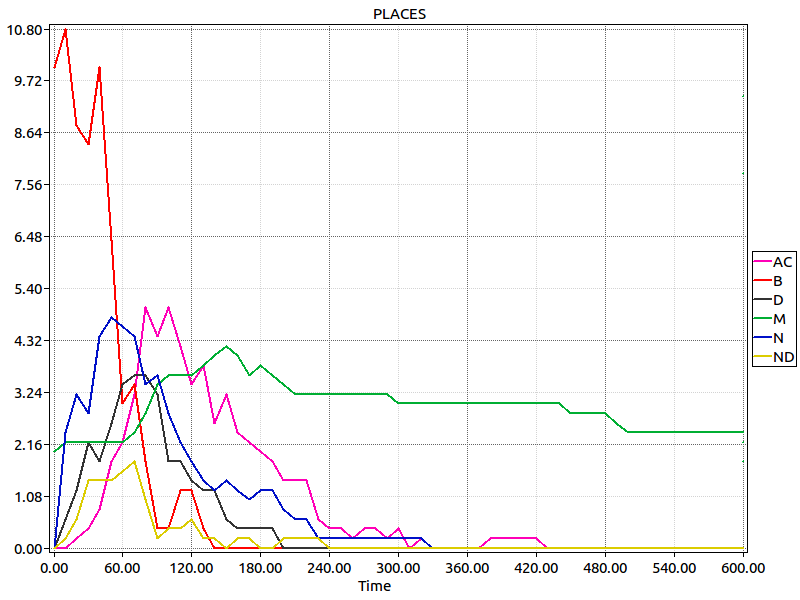
\includegraphics[scale=0.45]{imagens/resultados/RedeB_N_M_D_AC_27-02_v3-BacteriaElimination-NormalResponsefig1_PLACES.png}
			\end{center}
			\caption{Eliminação das bactérias e resolução da inflamação na rede de Petri com dano tecidual. 
			As citocinas anti-inflamatórias (AC) são representadas pela linha rosa. As bactérias (B) estão representadas em vermelho. 
			O dano tecidual (D) é representado pela linha na cor preta. Os macrófagos (M) estão representados pela cor verde. 
			A cor azul representa os neutrófilos (N) e a cor amarela representa os neutrófilos apoptóticos (ND).  }
			\label{cenario1}
		\end{figure}
		
		O cenário 2 que simula a depleção dos macrófagos tenta ilustrar a importância desse tipo de célula na regulação e resolução da resposta imune. 
		Para simular esse cenário, as taxas das funções de transição $M\_Migration1$ e $M\_Migration2$ foram diminuídas, sendo consideradas taxas três vezes menor 
		do que as do cenário 1. O resultado desse cenário é mostrado na Figura \ref{cenario2}. 
		
		\begin{figure}
			\begin{center}
				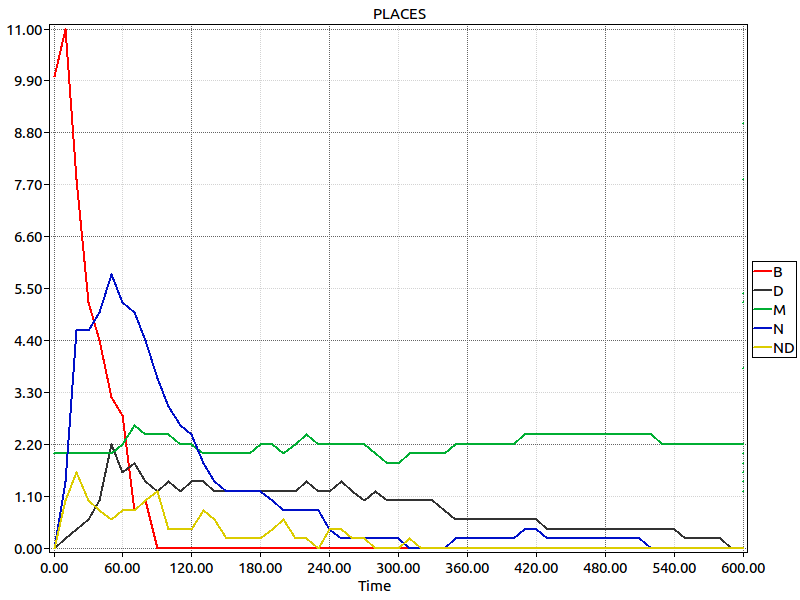
\includegraphics[scale=0.45]{imagens/resultados/RedeB_N_M_D_AC_27-02_v3-MacrophageDepletion-fig2_PLACES.png}
			\end{center}
			\caption{ }
			\label{cenario2}
		\end{figure}
		
		Observa-se, na Figura \ref{cenario2}, durante um tempo considerável após a eliminação das bactérias, a presença de dano tecidual e de neutrófilos, 
		ilustrando o fato de que a inflamação demorou a ser controlada. 
		Isso se deve ao fato de que há menos macrófagos migrando para controlar a inflamação. Os poucos macrófagos presentes no tecido demoram a realizar a limpeza 
		do local infectado (através da fagocitose de células mortas e de neutrófilos apoptóticos). Como consequência da inflamação persistente, há uma segunda 
		onda de migração de neutrófilos, por volta do instante de tempo $t=340$, atraídos pela inflamação. Por fim, próximo do tempo $t = 600$, 
		a inflamação cessa. 
		
		No cenário 3, temos a depleção de neutrófilos e macrófagos. O resultado para esse cenário é mostrado na Figura \ref{cenario3}. 
		Pode-se observar que, em relação aos outros cenários, a resposta imune levou um tempo maior para eliminar as bactérias. 
		Isso ocorreu porque poucos neutrófilos e macrófagos migram para o local infectado. Eles não são capazes de conter a infecção 
		durante um bom tempo. 
		% Como consequência disso, o dano tecidual 
		
		\begin{figure}
			\begin{center}
				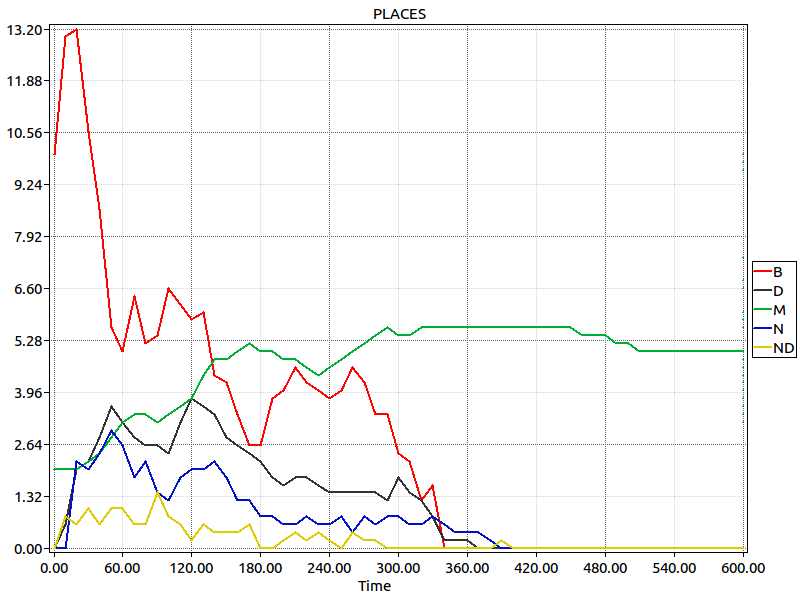
\includegraphics[scale=0.45]{imagens/resultados/RedeB_N_M_D_AC_27-02_v4-Leukocytedepletion-fig1_PLACES.png}
			\end{center}
			\caption{ }
			\label{cenario3}
		\end{figure}
		
		%Falar do impacto de considerar a influência da bactéria na migração dos macrófagos também. 
		
% 		Um dos resultados obtidos para o cenário 2 é mostrado na Figura ... 
% 		Observa-se que as bactérias apresentam um grande decrescimento no início, mas elas só são eliminadas depois do tempo $t=800$. 
% 		Um dos motivos é que os neutrófilos que migram para o tecido não são suficientes para conter a infecção bacteriana. Além disso, as bactérias causam um grande 
% 		dano tecidual que atrapalha a resposta imune, mas devido à limpeza realizada pelo macrófagos eliminando células mortas, a resposta imune consegue 
% 		eliminar as bactérias. 
						
		%A partir das simulações feitas observou-se que foi mais difícil obter a eliminação das bactérias para os cenários 1 e 2. 
		
	\section{Conclusão}  % e trabalhos futuros
	
	Neste trabalho, desenvolveu-se redes de Petri para a modelagem da resposta imune inata. Foi poss\'ivel modelar 
	diversos processos presentes nas respostas imunes atrav\'es da definiç\~ao de funç\~oes de transiç\~ao 
	nas transiç\~oes estocásticas e da utilizaç\~ao de arcos padr\~oes e arcos modificadores. 
	
	O software Snoopy facilitou e acelerou o processo de construç\~ao e simulaç\~ao das redes de Petri, permitindo, 
	entre outros recursos, a visualização da rede, visualização dos resultados da simulaç\~ao e um passo a passo 
	da execução da rede atrav\'es de uma animaç\~ao. 
	
	A partir das simulaç\~oes realizadas, observou-se a importância da transiç\~ao Inflammation\_Migration no 
	surgimento de um estado de inflamação cr\^onica. A presença de um \textit{feedback} positivo entre o dano 
	tecidual, neutr\'ofilos e macr\'ofagos modelando a migração de c\'elulas do sistema imune devido a efeitos 
	da inflamação enfatiza a importância do controle da inflamação que evita um estado de inflamação persistente. 
	Tamb\'em observou-se, a partir da an\'alise dos resultados, que o dano tecidual/inflamação persiste se existe 
	algum preju\'izo nas funç\~oes dos macr\'ofagos. 
	
	
% Pretendemos considerar, em nosso modelo, o uso pelas bactérias \ textit {S. aureus} dos seus sistemas sensoriais / reguladores
% para adaptar a produção de factores de virulência, especificamente a um sinal de activação, por exemplo, neutrófilos \ citep {Guerra2017}.
% A idéia é estudar como a interação entre \ textit {S. aureus} e neutrófilos provoca certa
% de respostas sensoriais e adaptativas usadas por \ textit {S. aureus} \ citep {Guerra2017}.
		
% 		Neste trabalho, foram desenvolvidas redes de Petri coloridas estocásticas para a modelagem da resposta 
% 		imune inata a uma infecção bacteriana. As redes desenvolvidas foram capazes de capturar comportamentos relevantes que são 
% 		observados durante a resposta imune a uma infecção bacteriana. 
		%Dentre esses comportamentos, destaca-se a importância do macrófago na resolução da resposta imune evitando um estado de inflamação persistente. 
		% Observou-se que a transição Inflammation\_Migration é importante para evitar um estado de inflamação crônica através 
		% do recrutamento de macrófagos 
	% para realizar a limpeza do local infectado. 
	
		% Redes de Petri são uma ferramenta poderosa para estudar sistemas complexas. 
		
% Bacteria adapt to environmental stresses imposed by the host by entering a different physiologic state. A key element of this different physiologic state is a non-replicating or slowly replicating growth rate, which may have the additional benefit of contributing to a pathogen’s defense against antibiotic exposure. 
				
% [Artigo Persistent bacterial infections, antibiotic tolerance, and the oxidative stress response]
% Numerous factors contribute to the difficulty in sterilizing persistent infections. One contributing factor may be that bacteria often establish persistent infections 
% within a “protected niche” in the host. For example, there are specific regions within the host where physical structures may obstruct an effective immune response and 
% prevent adequate penetration with antibiotics, notably the blood-brain barrier, joint spaces and the sinuses. In other cases, the host immune response may actually create 
% a “protected niche” by attempting to sequester the bacteria, exemplified by granulomas. While granuloma formation during M. tuberculosis infection represents a mechanism 
% of host-defense, granulomas are also believed to protect bacteria, though incompletely, from antibiotics. Finally, some pathogens may develop their own “protected niche,” 
% either through the formation of bacterial communities known as biofilms or by adapting to intracellular growth. 

% [Artigo With Friends Like These: The Complex Role of Neutrophils in the Progression of Severe Pneumonia]
% Neutrophil Resolution: 
% Equally important to neutrophil mediated immunity is the appropriate resolving of neutrophils in the lung. 
% This requires effective coordination of the termination of excessive neutrophil influx and the clearance of apoptotic neutrophils by efferocytosis. These processes are mediated in part by the biosynthesis of specialized pro-resolving mediators such as resolvins, or the presence of other molecules produced by host tissue including extracellular adenosine that signal the need to terminate and resolve an active inflammatory process (Serhan et al., 2002, 2014; Chiang et al., 2012; Bou Ghanem et al., 2015). Neutrophil turnover, specifically by constitutive apoptotic cell death, is an important part of effective pulmonary immunity. Delayed neutrophil death can exacerbate inflammation by increasing neutrophil numbers and therefore their propensity to cause significant tissue damage via the continuous release of toxic ROS, enzymes, and other antimicrobial factors. Effective control of neutrophil cell death is therefore essential to appropriate immune control and resolution of inflammation.
		
		
	 %TRABALHOS FUTUROS: 
		%Trabalhos futuros: acrescentar células do sistema adaptativo para modelar outros aspectos importantes 
		%nas infecções crônicas. Compreender melhor como algumas bactérias ... 
		 
		% We plan to consider, in our model, the use by the bacteria \textit{S. aureus} of its sensory/regulatory systems 
% to adapt the production of virulence factors, specifically to a triggering signal, e.g., neutrophils \citep{Guerra2017}. 
% The idea is to study how the interaction between \textit{S. aureus} and neutrophils provokes certain 
% sensing and adaptive responses used by \textit{S. aureus} \citep{Guerra2017}. 


    \bibliographystyle{unsrt}
    \bibliography{bibtex/relatorio}


\end{document}